\documentclass[a4paper,12pt,reqno]{amsart}
\usepackage{graphicx}
\usepackage{macros_M53}

% pour voir les solutions il faut enlever le commentaire de la ligne suivante
% \solutionstrue

\begin{document}

% ==================================
\hautdepage{

\ifsolutions{Solutions de l'examen final}\else{Examen final}\fi\par\normalfont\normalsize
4 janvier 2017\\{[ durée: 3 heures ]}\par
}
% ==================================
\ifsolutions\else
% {\fontencoding{U}\fontfamily{futs}\selectfont\char 66\relax}
\tikz[baseline=(e.base)]{\NoAutoSpacing\node(e){!};\draw[red,ultra thick,line join=round,yshift=-.15ex](90:1em)--(210:1em)--(330:1em)--cycle;}
\textbf{Documents autorisés :}\textit{Une feuille A4 recto-verso écrite à la main.}
\tsvp
\vspace*{\fill}
\fi


%-----------------------------------
\begin{exo} (Coniques)

  On se place dans $\mathbb{R}^{2}$ avec la structure euclidienne standard, dont la distance est notée $\d$. On considère une ellipse $\ens{E}$ qui n'est pas un cercle.

  \begin{enumerate}
    \item\label{M1M2} Montrer qu'il existe une unique paire de points $\{M_{1},M_{2}\}$ tel que
    \[
      \d(M_{1},M_{2})=\max_{A,B \in \ens{E}}\d(A,B).
    \]
    \item\label{S1S2}
    \begin{minipage}[t]{.7\linewidth}
      Soit $\id$ l'identité de $\mathbb{R}^{2}$, $S_{1}$ la symétrie orthogonale par rapport à la droite $\affspan{M_{1},M_{2}}$ et $S_{2}$ la symétrie orthogonale par rapport à la médiatrice de $[M_{1},M_{2}]$. En déduire que l'ensemble des isométries affines qui préservent $\ens{E}$, c'est-à-dire les $\phi \in \iso{\mathbb{R}^{2}}$ telles que $\phi(\ens{E})=\ens{E}$, est
      \[
        \{\id,\, S_{1},\, S_{2},\, S_{1}S_{2}\}.
      \]
    \end{minipage}\hfill
    \begin{minipage}[t]{.28\linewidth}~\\
      \hspace*{\fill}
      \scalebox{.77}{\input{M53_2016-17_DS2_exo1.tikz}}
    \end{minipage}
    \item Préciser la nature et les paramètres de $S_{1}S_{2}$.
  \end{enumerate}

  Pour la suite de l'exercice on considère l'ensemble
    \[
      \ens{E}=\{ (x,y) \in \mathbb{R}^{2} \mid 4(x+y-4)^{2}+(x-y)^{2}=16\}.
    \]

  \begin{enumerate}[resume]
    \item Montrer que $\ens{E}$ est une ellipse.\\
    \begin{indication}
      Au vu de la forme de l'équation, on peut envisager un changement de variables de la forme $X=\frac{1}{\sqrt{2}}(x+y-4)$ et $Y=\frac{1}{\sqrt{2}}(x-y)$. Le cas échéant, il faut justifier son utilisation.
    \end{indication}
    \item Déterminer les coordonnées cartésiennes dans le repère canonique des deux points $M_{1}$ et $M_{2}$ définis dans la question \eqref{M1M2}.\\
    \item Écrire les expressions analytiques dans le repère canonique des deux symétries $S_{1}$ et $S_{2}$ définies dans la question \eqref{S1S2}.
  \end{enumerate}

\end{exo}

\begin{solution}
  \begin{enumerate}
    \item
    \begin{minipage}[t]{.77\linewidth}
      D'après le cours, comme $\ens{E}$ n'est pas un cercle, il existe deux points (les foyers) $F_{1}$ et $F_{2}$ et une constante $a > d(F_{1},F_{2})/2$ tels que $\ens{E} = \{M \in \mathbb{R}^{2}\,\mid\, d(F_{1},M) + d(M,F_{2}) = 2a\}$. Soient $M_{1}$ et $M_{2}$ les deux points de E situés sur l'axe focal, c'est à dire alignés avec $F_{2}$ et $F_{2}$.
    \end{minipage}\hfill
    \begin{minipage}[t]{.21\linewidth}~\\[14mm]
      \hspace*{\fill}
      \smash{\scalebox{.7}{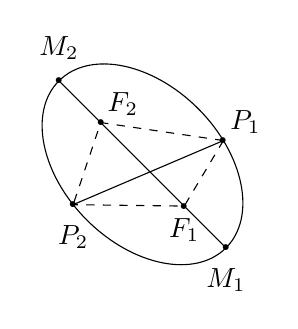
\begin{tikzpicture}[rotate=-45,xscale=1.5]
	\path 
		(0:1) coordinate (M1) node[scale=2]{.} node[below=4pt]{$M_1$}
		(180:1) coordinate (M2) node[scale=2]{.} node[above=4pt]{$M_2$}
		(0:.5) coordinate (F1) node[scale=2]{.} node[below=1pt]{$F_1$}
		(180:.5) coordinate (F2) node[scale=2]{.} node[above right=-1pt]{$F_2$}
		(70:1) coordinate (P1) node[scale=2]{.} node[above right=-1pt]{$P_1$}
		(-100:1) coordinate (P2) node[scale=2]{.} node[below=4pt]{$P_2$}
		;
		
	\draw 
		circle(1)
		(M1) -- (M2)
		(P1) -- (P2)	
	;	
	\draw[dashed]
		(P1) -- (F1) -- (P2)
		(P1) -- (F2) -- (P2)
	;
\end{tikzpicture}
}}
    \end{minipage}\\[3mm]
    Soient $P_1$ et $P_2$ deux  points de $\ens{E}$, alors pour $i=1,2$ on a $d(P_{1},P_{2}) \leq d(P_{1},F_{i}) + d(F_{i},P_{2})$ avec égalité si et seulement si $P_{1}, P_{2}$ et $F_{i}$ sont alignés. En sommant ces deux inégalités on trouve $d(P_{1},P_{2}) \leq 4a$ avec égalité si et seulement si $P_{1}$, $ P_{2}$, $F_{1}$ et $F_{2}$  sont alignés, autrement dit si et seulement si $\{P_{1},P_{2}\} = \{M_{1},M_{2}\}$.
    \item
    \begin{minipage}[t]{.77\linewidth}
      D'après la question précédente toute isométrie $\phi$ qui préserve $\ens{E}$ préserve $\{M_{1},M_{2}\}$. Ainsi elle admet un point fixe $\Omega = \frac{1}{2} M_{1} + \frac{1}{2} M_{2}$ et préserve la médiatrice de $[M_{1},M_{2}]$ comme le lieu des points équidistants de $M_{1}$ et $M_{2}$. Notons $[N_{1},N_{2}]$ les deux points d'intersection de la médiatrice avec $\ens{E}$, qui forment également un couple de points préservé par $\phi$, comme intersection de deux ensembles préservés par $\phi$.
    \end{minipage}\hfill
    \begin{minipage}[t]{.21\linewidth}~\\[21mm]
      \hspace*{\fill}
      \smash{\scalebox{.7}{\begin{tikzpicture}
	\path 
		(3,1) coordinate (M1) node[scale=2]{.} node[below=4pt]{$M_1$}
		(1,3) coordinate (M2) node[scale=2]{.} node[above=4pt]{$M_2$}
		({2-1/sqrt(2)},{2-1/sqrt(2)}) coordinate (N1) node[scale=2]{.} node[below=4pt]{$N_1$}
		({2+1/sqrt(2)},{2+1/sqrt(2)}) coordinate (N2) node[scale=2]{.} node[above=4pt]{$N_2$}
		(2,2) coordinate (Omega) node[scale=2]{.} node[above=4pt]{$\Omega$};
	\draw [rotate=-45, shift={($(M1)!.5!(M2)$)}]ellipse(1.41421356237cm and 1cm);	
	\draw 
		($(M1)!1.5!(M2)$) -- ($(M2)!1.5!(M1)$) coordinate (S1) node[above right] {$S_1$}
		($(M1)!.5!(M2)!2!90:(M2)$) -- ($(M2)!.5!(M1)!2!90:(M1)$) coordinate (S2) node[below right] {$S_2$};
	\draw[swap/.style={latex-latex, bend right}] 
		([shift={(90:.4)}]S1) edge[swap] ([shift={(0:-.4)}]S1)
		([shift={(180:.4)}]S2) edge[swap] ([shift={(90:-.4)}]S2);
\end{tikzpicture}
}}
    \end{minipage}\\[2.1mm]
    Comme $\Omega$, $M_{1}$ et $N_{1}$ ne sont pas alignés, ils forment un repère affine de $\mathbb{R}^{2}$. Ainsi $\phi$ est complètement déterminée par l'image de ce repère.\\
    D'après ce qu'on a vu $\phi(\Omega) = \Omega$, $\phi(M_{1}) \in \{M_{1},M_{2}\}$ et $\phi(N_{1}) \in \{N_{1},N_{2}\}$. Ainsi il ne peut y avoir qu'au plus $4$ isométries qui préservent $\ens{E}$. Maintenant il est facile de voir que les $4$ isométries de l'énoncé conviennent :
    \begin{align*}
      \id(M_{1})=M_{1}&,\quad \id(N_{1})=N_{1}, &
      S_{1}(M_{1})=M_{1}&,\quad S_{1}(N_{1})=N_{2}, \\
      S_{2}(M_{1})=M_{2}&,\quad S_{2}(N_{1})=N_{1}, &
      S_{1}S_{2}(M_{1})=M_{2}&,\quad S_{1}S_{2}(N_{1})=N_{2}.
    \end{align*}
    \item Comme les axes des deux symétries $S_{1}$ et $S_{2}$ sont orthogonaux, leur composée est une rotation de $2\times \pm \dfrac{\pi}{2} = \pm \pi$, autour de leur intersection $\Omega$. Autrement dit $S_{1}S_{2}$ est une symétrie centrale de centre $\Omega$.
    \item Comme l'application $(x,y) \mapsto \big(\,\frac{1}{\sqrt{2}}(x+y-4),\,\frac{1}{\sqrt{2}}(x-y)\,\big)$ est une isométrie affine de partie linéaire la réflexion ayant pour matrice dans la base canonique
    $
      \begin{psmallmatrix}
        \frac{1}{\sqrt{2}} & \frac{1}{\sqrt{2}} \\
        \frac{1}{\sqrt{2}} & -\frac{1}{\sqrt{2}} \\
      \end{psmallmatrix}
    $, alors le changement de coordonnées proposé dans l'indication correspond à un autre repère cartésien orthonormé $\mathcal{R}$ dans lequel l'équation de $\ens{E}$ devient
    \[
      \ens{E}=\{ (X,Y) \in \mathbb{R}^{2} \mid \big(\frac{X}{\sqrt{2}}^{2}\big)+\big(\frac{Y}{2\sqrt{2}}^{2}\big)=1\},
    \]
    qui est, d'après le cours, l'équation d'une ellipse de rayons $\sqrt{2}$ et $2\sqrt{2}$.
    \item D'après la question précédente le grand axe de $\ens{E}$ est l'axe des $Y$, et donc les points $M_{1}$ et $M_{2}$ ont pour coordonnées $(0,2\sqrt{2})_{\mathcal{R}}$ et $(0,-2\sqrt{2})_{\mathcal{R}}$ dans le repère $\mathcal{R}$. Ainsi en appliquant le changement de coordonnées inverse, $x=\frac{1}{\sqrt{2}}(X+Y)+2$ et $y=\frac{1}{\sqrt{2}}(X-Y)+2$, on trouve les coordonnées dans la base canonique $(4,0)$ et $(0,4)$.
    \item L'expression de $S_{1}$ dans le repère $\mathcal{R}$ est $S_{1}(X,Y)_{\mathcal{R}}=(-X,Y)_{\mathcal{R}}$. Ainsi en appliquant les changements de repère on trouve $S_{1}(x,y) = S_{1}\big(\frac{1}{\sqrt{2}}(x+y-4), \frac{1}{\sqrt{2}}(x-y)\big)_{\mathcal{R}} = (-\frac{1}{\sqrt{2}}(x+y-4), \frac{1}{\sqrt{2}}(x-y))_{\mathcal{R}} = (4-y, 4-x)$. De même on trouve $S_{2}(x,y)=(y,x)$.
  \end{enumerate}
\end{solution}

%-----------------------------------
\begin{exo} (Groupe d'isométries)

  On considère l'ensemble $\ens{T}$ à quatre points $A$, $B$, $C$ et $D$ de $\mathbb{R}^{3}$:
  \[
    \ens{T} = \big\{ A(1,0,0),\, B(2,0,0),\, C(1,1,0),\, D(1,0,1)\big\}.
  \]
  Décrire, en précisant leurs paramètres, les rotations qui préservent $\ens{T}$, c'est-à-dire les rotations $R$ telles que $R(\ens{T})=\ens{T}$.

  \begin{indication}
    Dessiner l'ensemble $\ens{T}$. Montrer qu'un des points de $\ens{T}$, à préciser, doit être fixe par ces rotations.
  \end{indication}
\end{exo}

\begin{solution}

  \begin{minipage}[t]{.70\linewidth}
    Nous avons
    \begin{gather*}
      d(A,B)=d(A,C)=d(A,D)=1, \\
      d(B,C)=d(C,D)=d(D,B)=\sqrt{2}.
    \end{gather*}
    Ainsi toute isométrie qui préserve les $4$ points doit envoyer $A$ en $A$ car c'est le seul point dont les distances aux autres points sont toutes égales à $1$.\\[-3mm]
  \end{minipage}\hfill
  \begin{minipage}[t]{.21\linewidth}~\\[21mm]
    \hspace*{\fill}
    \smash{\scalebox{.7}{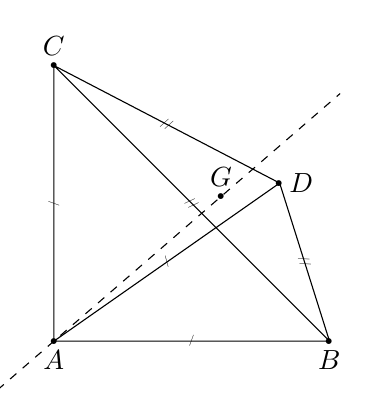
\begin{tikzpicture}[z={(35:1)},>=latex, scale=3.5]
	\path
		(1,0,0) coordinate (A) node[scale=2]{.} node[below]{$A$}
		(2,0,0) coordinate (B) node[scale=2]{.} node[below]{$B$}
		(1,1,0) coordinate (C) node[scale=2]{.} node[above]{$C$}
		(1,0,1) coordinate (D) node[scale=2]{.} node[right]{$D$}
		(4/3,1/3,1/3) coordinate (G) node[scale=2]{.} node[above]{$G$}
	;
		

	\draw 
		(A) -- node[scale=.4,sloped]{/} (B)
		(A) -- node[scale=.4,sloped]{/} (C)
		(A) -- node[scale=.4,sloped]{/} (D)
		(B) -- node[scale=.4,sloped]{//} (C)
		(C) -- node[scale=.4,sloped]{//} (D)
		(D) -- node[scale=.4,sloped]{//} (B)
	;
	\draw[dashed, shorten <=-2cm, shorten >=-2cm] (A) -- (G);
\end{tikzpicture}
}}
  \end{minipage}\\
  Et comme cette isométrie doit permuter $B$, $C$ et $D$ elle préserve leur isobarycentre $G(\frac{1}{3},\frac{1}{3},\frac{1}{3})$.
  \begin{minipage}[t]{.77\linewidth}
    Ainsi toute rotation qui préserve les $4$ points doit avoir comme axe la droite $\affspan{A,G}$ qui est orthogonale au plan $\affspan{B,C,D}$, comme hauteur dans un tétraèdre isocèle à base équilatérale. Et sa restriction au plan $\affspan{B,C,D}$ est une rotation qui permuter les sommets du triangle équilatéral $BCD$, donc doit être d'angle $0$, $\frac{2\pi}{3}$ ou $-\frac{2\pi}{3}$.\\[-3mm]
  \end{minipage}\hfill
  \begin{minipage}[t]{.21\linewidth}~\\[19mm]
    \hspace*{\fill}
    \smash{\scalebox{.77}{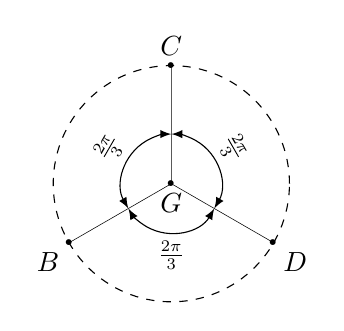
\begin{tikzpicture}[z={(35:1)},>=latex, scale=1.5]
	\path
		(0,0) node[scale=2]{.} node[below]{$G$}
		(210:1) coordinate (B) node[scale=2]{.} node[below left]{$B$}
		(90:1) coordinate (C) node[scale=2]{.} node[above]{$C$}
		(-30:1) coordinate (D) node[scale=2]{.} node[below right]{$D$}
	;
	\draw[dashed, shorten <=-2cm, shorten >=-2cm] circle(1);
	\draw[very thin]
		(0,0) -- (B)
		(0,0) -- (C)
		(0,0) -- (D)
	;
	\draw[latex-latex] (-30:.42) arc(-30:90:.42) node[pos=.5,above,sloped,scale=.84]{$\frac{2\pi}{3}$};
	\draw[latex-latex] (210:.42) arc(210:90:.42) node[pos=.5,above,sloped,scale=.84]{$\frac{2\pi}{3}$};
	\draw[latex-latex] (-30:.42) arc(-30:-150:.42) node[pos=.5,below,sloped,scale=.84]{$\frac{2\pi}{3}$};
\end{tikzpicture}
}}
  \end{minipage}\\
  Et réciproquement toute rotation d'axe $\affspan{A,G}$ et dont la restriction à $\affspan{B,C,D}$ est une rotation de $0$, $\frac{2\pi}{3}$ ou $-\frac{2\pi}{3}$ autour de $G$ convient clairement car elle permute $B,C,D$ et préserve~$A$.
\end{solution}

%-----------------------------------
\begin{exo} (Espaces affines)

  On considère le sous-ensemble $\ens{P} \subset \mathbb{R}_{2}[X]$ des polynômes de degré au plus $2$ qui vérifient l'équation
  \[
    \int_{0}^{1}Q(t)\operatorname{d}\!t=1.
  \]
  \begin{enumerate}
    \item Montrer que $\ens{P}$ est un sous-espace affine de l'espace vectoriel $\mathbb{R}_{2}[X]$. Préciser un point de $\ens{P}$, ainsi que sa direction $\ev{P}$.
    \item Donner un repère cartésien et un repère affine de $\ens{P}$.
  \end{enumerate}

  % On considère l'ensemble $\ens{R}$ des suites récurrentes réelles qui vérifient
  % \[
  %   u_{n+2} = 3 u_{n+1} - 2 u_{n} +1.
  % \]
  % \begin{enumerate}
  %   \item Montrer que $\ens{R}$ est un sous-espace affine de l'espace vectoriel $\mathbb{R}^{\mathbb{N}}$ des suites réelles. Préciser un point de $\ens{R}$, ainsi que sa direction $\ev{R}$.

  %   \begin{indication}
  %     Chercher une suite de $\ens{R}$ de la forme $u_{n}=an$.
  %   \end{indication}
  %   \item Donner un repère cartésien et un repère affine de $\ens{R}$.
  % \end{enumerate}

\end{exo}

\begin{solution}
  \begin{enumerate}
    \item Comme l'intégrale $Q \mapsto \int_{0}^{1}Q(t)\operatorname{d}\!t $ est une application linéaire sur $\mathbb{R}_{2}[X]$, notons la $I$, alors $\ens{P}=I^{-1}(1)$ est un sous espace affine de $\mathbb{R}_{2}[X]$ de direction $\ev{P}=I^{-1}(0)$, les polynômes à intégrale $0$. Nous avons $\int_{0}^{1}1\operatorname{d}\!t=1$, donc le polynôme constant $1$ est un élément de $\ens{P}$.
    \item Soit $Q(X)=aX^{2}+bX+c$, alors $\int_{0}^{1}Q(t)\operatorname{d}\!t=\frac{a}{3}+\frac{b}{2}+c$, et donc $\ev{P} = \{aX^{2}+bX+c \,\mid\, \frac{a}{3}+\frac{b}{2}+c=0\}=\affspan{3X^{2}-1, 2X-1}$. Ainsi un repère cartésien de $\ens{P}$ est $\left(1,3X^{2}-1,2X-1\right)$, et un repère affine est $\left(1,3X^{2},2X\right)$.
  \end{enumerate}
\end{solution}

%-----------------------------------
\begin{exo} (Géométrie dans le plan complexe)

  On se place dans le plan complexe.
  \begin{enumerate}
    \item Indiquer sur un dessin la position des points dont les affixes sont les racines de l'équation $z^{2}+z+1=0$.
    \item Soit $A$, $B$ et $C$ trois points du plan complexe d'affixes respectives $a$, $b$ et $c$. Montrer que le triangle $ABC$ est équilatéral si et seulement si
    \begin{equation}\label{eq:triangle}
      a\mu^{2}+b\mu+c=0\tag{$\bigtriangleup$}
    \end{equation}
    pour $\mu$ une des racines de $z^{2}+z+1=0$.
  \end{enumerate}
  \begin{enumerate}[resume]
    \item Soit $a=-2i$ l'affixe de $A$ et $b=1+i$ l'affixe de $B$. Déterminer les affixes $c$ des points $C$ tels que le triangle $ABC$ soit équilatéral.\\[-4mm]
    \item
    \begin{minipage}[t]{.56\linewidth}
      Soit $ABC$ un triangle équilatéral tel que l'affixe de son centre soit $0$ et l'affixe de $C$ soit $i$. Déterminer les affixes des trois centres des cercles exinscrits de $ABC$ et vérifier qu'elles vérifient l'équation \eqref{eq:triangle}.\\
      \begin{indication}
        Il y a une relation directe entre l'affixe d'un sommet du triangle et l'affixe du centre du cercle exinscrit opposé.
      \end{indication}
    \end{minipage}\hfill
    \begin{minipage}[t]{.42\linewidth}~\\[11mm]
      \hspace*{\fill}
      \smash{\scalebox{.7}{\tikzset{
	longer/.style = {
		shorten <= -2cm,
		shorten >= -2cm
	}
}
\begin{tikzpicture}[scale=1.4,baseline=0pt]
	\path
		[inner sep=2]
		(90:1) coordinate (C) node[scale=2, label={90:$C$}]{.}
		[inner sep=1]
		(-30:1) coordinate (B) node[scale=2,label={-15:$B$}]{.}
		(-150:1) coordinate (A) node[scale=2, label={195:$A$}]{.}
		[inner sep=.5]
		(90:-2) coordinate (OC) node[scale=2, label={-90:$O_C$}]{.}
		(-30:-2) coordinate (OB) node[scale=2, label={105:$O_B$}]{.}
		(-150:-2) coordinate (OA) node[scale=2, label={15:$O_A$}]{.}
		(0:0) coordinate (O) node[scale=2, label={90:$O$}]{.}
	;
	\draw (A) edge[longer] (B) (B) edge[longer] (C) (C) edge[longer] (A);
	\draw[dashed]
		(OA) circle (1.5)
		(OB) circle (1.5)
		(OC) circle (1.5)
	;

\end{tikzpicture}
}}
    \end{minipage}
  \end{enumerate}

\end{exo}

\begin{solution}
  \begin{enumerate}
    \item
    Les deux racines de l'équation sont habituellement notées $j=e^{\frac{2i\pi}{3}}=-\frac{1}{2}+i\frac{\sqrt{3}}{2}$ et $\bar{j}=e^{\frac{-2i\pi}{3}}=-\frac{1}{2}-i\frac{\sqrt{3}}{2}$ et nous avons $j^{2}=\bar{j}$ et $\bar{j}^{2}=j$.
    \begin{center}
      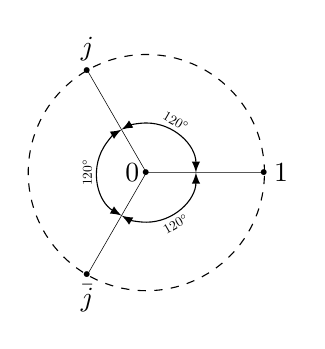
\begin{tikzpicture}[z={(35:1)},>=latex, scale=1.5]
	\path
		(0,0) coordinate (0) node[scale=2]{.} node[left=-1pt]{$0$}
		(0:1) coordinate (1) node[scale=2]{.} node[right]{$1$}
		(120:1) coordinate (j) node[scale=2]{.} node[above]{$j$}
		(-120:1) coordinate (jb) node[scale=2]{.} node[below]{$\bar{j}$}
	;
	\draw[dashed, shorten <=-2cm, shorten >=-2cm] circle(1);
	\draw[very thin]
		(0,0) -- (1)
		(0,0) -- (j)
		(0,0) -- (jb)
	;
	\draw[latex-latex] (0:.42) arc(0:120:.42) node[pos=.5,above,sloped,scale=.49]{$120^{\circ}$};
	\draw[latex-latex] (240:.42) arc(240:120:.42) node[pos=.5,above,sloped,scale=.49]{$120^{\circ}$};
	\draw[latex-latex] (0:.42) arc(0:-120:.42) node[pos=.5,below,sloped,scale=.49]{$120^{\circ}$};
\end{tikzpicture}

    \end{center}
    \item $ABC$ est un triangle équilatéral si et seulement si le vecteur $\vv{AC}$ est l'image par rotation de $\pm \frac{\pi}{3}$ du vecteur $\vv{AB}$, autrement dit si et seulement si $\vv{AC}$ est l'image par rotation de $\pm \frac{2\pi}{3}$ du vecteur $\vv{BA}$. En exprimant ceci en termes d'affixes, nous constatons que $ABC$ est équilatéral si et seulement si $(c-a)=e^{\pm\frac{2i\pi}{3}}(a-b)$ $\Leftrightarrow$ $a(-1-\mu)+b\mu+c=0$ où $\mu=e^{\pm\frac{2i\pi}{3}}$ est l'une des racines $j$ ou $\bar{j}$. Pour finir il suffit de remarquer que $-1-\mu=\mu^{2}$.
    \item D'après la question précédente les affixes de $c$ possibles sont $c=-a \mu^{2} - b \mu$ où $\mu$ est l'une des racines $j$ ou $\bar{j}$. Ainsi $c=-(-2i)(-\frac{1}{2}\mp i\frac{\sqrt{3}}{2}) - (1+i) (-\frac{1}{2}\pm i\frac{\sqrt{3}}{2}) = \frac{1}{2} \pm \frac{3\sqrt{3}}{2} + i(-\frac{1}{2}\mp\frac{\sqrt{3}}{2})$.
    \item Les affixes de $A$ et $B$ sont obtenues en multipliant par $j$ et $\bar{j}$ l'affixe de $C$, car ces points sont l'image de $C$ par rotation de $\pm \frac{2\pi}{3}$. Ainsi les trois affixes de $A$, $B$ et $C$ sont $ji$, $\bar{j}i$ et~$i$.\\
    \begin{minipage}[t]{.7\linewidth}
      Comme $BO_{A}$ et $CO_{A}$ sont des bissectrices des angles extérieurs, on trouve les mesures des angles $\widehat{CBO_{A}}=\widehat{BCO_{A}}=60°$ et donc le triangle $BCO_{A}$ est également équilatéral. Ainsi le centre $O$ du triangle $ABC$ est sur le segment $AO_{A}$ et le coupe en rapport $\frac{1}{3}:\frac{2}{3}$ (voir la figure). Et comme l'affixe de $O$ est $0$ on trouve que l'affixe de $O_{A}$ est $(-2)$ $\times$ (l'affixe de $A$). De même, les affixes de $O_{B}$ et $O_{C}$ sont obtenues en multipliant par $(-2)$ les affixes de $B$ et $C$ respectivement. Ainsi les trois affixes sont $-2ji$, $-2\bar{j}i$ et $-2i$.
    \end{minipage}\hfill
    \begin{minipage}[t]{.28\linewidth}~\\[28mm]
      \hspace*{\fill}
      \smash{\scalebox{.7}{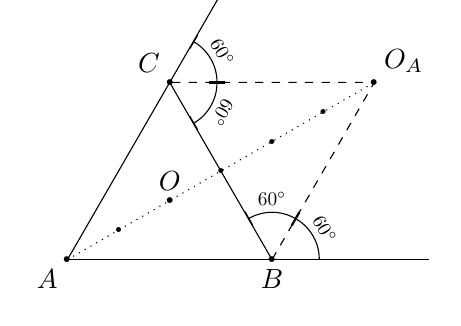
\begin{tikzpicture}[z={(35:1)},>=latex, scale=1.5]
	\path
		(0,0) coordinate (0) node[scale=2]{.} node[above]{$O$}
		(-150:1) coordinate (A) node[scale=2]{.} node[below left]{$A$}
		(-30:1) coordinate (B) node[scale=2]{.} node[below]{$B$}
		(90:1) coordinate (C) node[scale=2]{.} node[above left]{$C$}
		(30:2) coordinate (OA) node[scale=2]{.} node[above right]{$O_A$}
		(-150:.5) coordinate (0) node[scale=1.7]{.}
		(30:.5) coordinate (0) node[scale=1.7]{.}
		(30:1) coordinate (0) node[scale=1.7]{.}
		(30:1.5) coordinate (0) node[scale=1.7]{.}
	;
	\draw[shorten >= -2cm] (A) -- (B); 
	\draw[shorten >= -2cm] (A) -- (C);
	\draw (C) -- (B);
	\draw[dashed] (B) -- (OA) --(C);
	\draw[dotted] (A) -- (OA);
	
	\draw[|-|, shift={(B)}] (0,0) ++(0:.4) arc(0:60:.4) node[pos=.5, sloped, scale=.7, above]{$60^{\circ}$};
	\draw[|-|, shift={(B)}] (0,0) ++(60:.4) arc(60:120:.4) node[pos=.5, sloped, scale=.7, above]{$60^{\circ}$};
	\draw[|-|, shift={(C)}] (0,0) ++(0:.4) arc(0:60:.4) node[pos=.5, sloped, scale=.7, above]{$60^{\circ}$};
	\draw[|-|, shift={(C)}] (0,0) ++(0:.4) arc(0:-60:.4) node[pos=.5, sloped, scale=.7, swap, above, allow upside down]{$60^{\circ}$};
\end{tikzpicture}
}}
    \end{minipage}\\[3mm]
    Pour finir, comme les affixes de $ABC$ vérifient \eqref{eq:triangle}, en  multipliant par $(-2)$ l'équation, on trouve que les affixes de $O_{A}$, $O_{B}$ et $O_{C}$ vérifient aussi \eqref{eq:triangle}.

  \end{enumerate}
\end{solution}


\end{document}
